Deep End-to-end Causal Inference ("DECI", \cite{geffner2022deep})
\footnote{\url{https://github.com/microsoft/causica/}}
is an autoregressive-flow based non-linear additive noise structural equation model (SEM), which is designed to perform both causal discovery and inference, including average treatment effect (ATE) and conditional average treatment effect (CATE) estimation. DECI discovery takes prior knowledge of the graph structure as input, defined by a constraint adjacency matrix, and uses the data-driven causal calculation to estimate the graph structure and ATE between nodes.

\subsection{Using DECI for Timeseries: A Featurization Method}

\textit{SimSim-DECI} uses the DECI model to simulate temporal records for the patients under various drug-dose policies and finds the policy for the optimum dosage level. DECI is primarily designed to digest generic types of tabular datasets. To capture the temporal dynamics of our data, we designed our framework as follows:

\begin{itemize}
\item \textit{Temporal Sliding-Window featurization}: each row contains the information of the current time-step and the previous one as in \((X_{t-1},X_{t})\). Figure \ref{fig:temporal_featurized} shows what re-framed dataset looks like.

\item \textit{Temporal constraints}: Features in the current steps cannot cause features in the previous step.

\item \textit{Temporal training}: The DECI model is trained on each row as an independent sample. Since each row holds the past and current features, the connection between features of the same day is learned as well as features of two consecutive days.

\item \textit{Temporal simulation}: We simulate the information of each step by conditioning the simulation on the information from the previous step. That means for data in Figure \ref{fig:temporal_featurized}, we take the values of the seven right columns as the condition for the intervention and predict the next step by sampling the trained model.
\end{itemize}

\begin{figure}
    \centering
    \includegraphics[width=0.95\textwidth]{figures/temporal_signal.png}
    \caption{Dataset is re-framed to capture temporal dynamics on each row.}
    \label{fig:temporal_featurized}
\end{figure}

\subsection{Causal Discovery}

DECI recovers the structure of the underlying causal graph that we can compare with the true underlying graph. Thus, we can be the expert-in-the-loop to modify the data-driven findings to improve its correspondence to the truth. We do this by re-training with additional constraints. Figure \ref{fig:discovered_graphs} shows the 
%discovered unconstrained graph compared to the 
final graph with expert-in-the-loop constraints applied. Note that the domain expert prevented \textit{confounding by indication} (\cite{kyriacou2016confounding}) by reversing the direction of drug-to-severity causality. % and retaining the drug\_prev-to-severity connection.

% \begin{figure}
%     \centering
%      \begin{subfigure}[b]{0.25\textwidth}
%          \centering
%          \includegraphics[width=\textwidth]{figures/noconstraint_graph_discovery.png}
%          \caption{No constraint}
%      \end{subfigure}
%      \begin{subfigure}[b]{0.35\textwidth}
%          \centering
%          \includegraphics[width=\textwidth]{figures/constrainted_v2_graph_discovery.png}
%          \caption{Expert-defined Constraints}
%      \end{subfigure}
%         \caption{Discovered graph by DECI with no constraint (left) vs. with prior constraints defined by Expert including temporal (right).}
%         \label{fig:discovered_graphs}
% \end{figure}

\begin{figure}
    \centering
    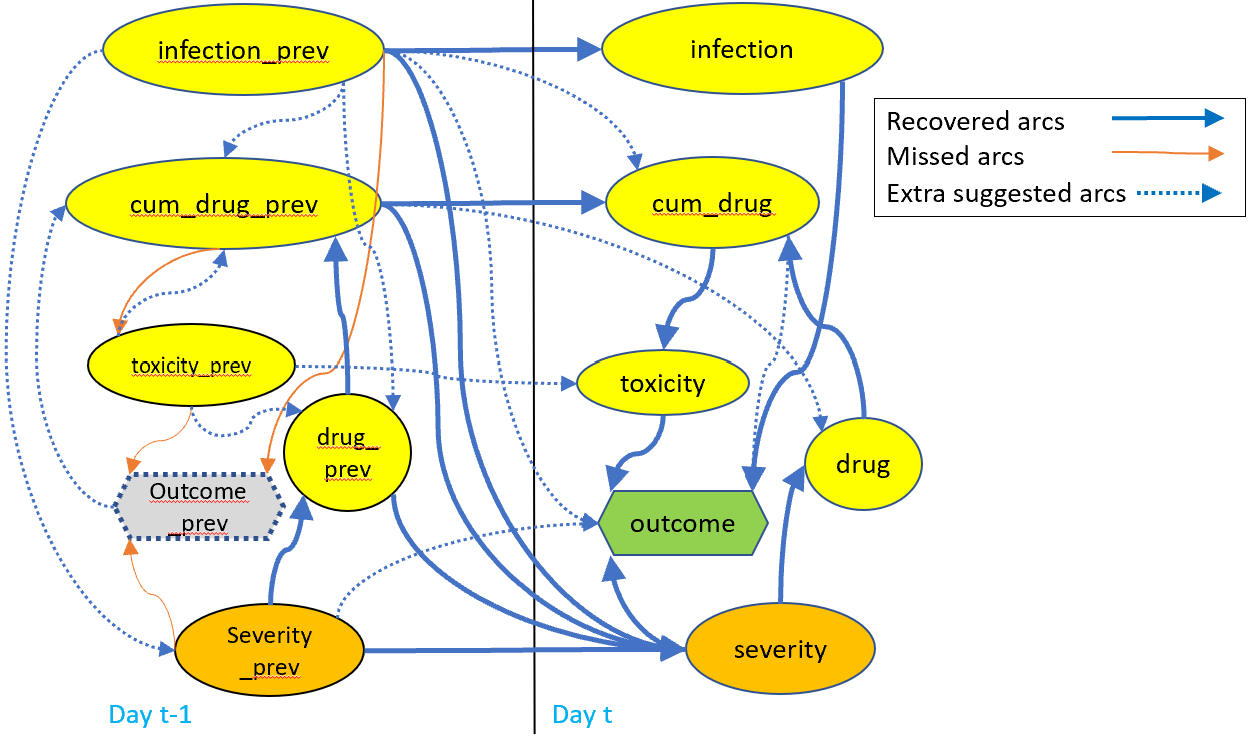
\includegraphics[width=0.8\textwidth]{figures/constrainted_graph_discovery_eval.png}
     \caption{The learned model with causal constraints. By adding structure constraints, DECI returns a model, which misses 4 arcs, but recovers 14 arcs. It also, suggests 11 extra arcs, which are not accurate based on the original model. Note, this 2-day graph is the equivalent to the original 3-day one on Figure \ref{fig:HBS_sequence}. This is possible because each feature only depends on features not more than one day away. Also, we do not need efficacy node as DECI can handle more complex inputs than the table-based Bayes net model used above.}
     %The effect of constraints are visible in the current Day $t$ timestep; the previous Day $t-1$ timestep does not have them by comparison, resulting in spurious dependencies.
        \label{fig:discovered_graphs}
\end{figure}

\subsection{Simulation-based Policy Optimization}

The trained model is a structural causal model (SCM) that captures the functional relations and error distributions. Hence, it is capable of estimating the expected updates following an intervention. We use this capability to synthesize the current day, having information about the previous day. We add the desired drug dose based on the candidate policies, explained in previous sections, to the interventions. To reduce estimation error, we take the average of 50 samples for the continuous variables and take the mode for the binary ones. The simulation for each patient will stop if ``die'' or ``recover'' returns True. Figure \ref{fig:optimizing_dose} demonstrates the results of different dose policies. The model captures the optimum drug dose correctly, although is less accurate at extremes where the observational data is sparse (see the "simsim-DECI" curve in Figure \ref{fig:optimizing_dose}). Note that this model is too optimistic about survival rates for intermediate doses; this may be because the learned graph did not find the edge from `cum\_drug' to 'efficacy', which reduces the benefit provided by the drug at moderate doses.

% \ref{fig:deci_dose_optimization}

% \begin{figure}
%     \centering
%     \includegraphics[width=0.8\textwidth]{figures/DoseOptimization.png}
%     \caption{We used the }
%     \label{fig:deci_dose_optimization}
% \end{figure}


% \subsection{Evaluation}
% Since we have knowledge of the ground-truth, we can evaluate the results from discovery, inference and policy optimization steps separately.  
